\documentclass[../notes.tex]{subfiles}

\pagestyle{main}
\renewcommand{\chaptermark}[1]{\markboth{\chaptername\ \thechapter\ (#1)}{}}
\setcounter{chapter}{4}

\begin{document}




\chapter{Exam and Molecular Spectroscopy}
\section{Intro to Molecular Spectroscopy}
\begin{itemize}
    \item \marginnote{2/2:}First half of the course: Techniques that apply to materials.
    \item Second half of the course: Techniques that apply to molecular systems, specifically bioinorganic ones.
    \item Less structural information now; more \textbf{spectroscopy}.
    \item \textbf{Spectroscopy}: The study of the interaction of light with \emph{molecular} systems.
    \item Today: Intro to spectroscopy (specifically vibrational) and group theory.
    \item Schedule after today:
    \begin{itemize}
        \item Magnetism (doesn't really involve radiation, but whatever).
        \item EPR, XAS, Mossbauer, elecrochemistry, NMR, and (time-permitting) some examples.
    \end{itemize}
    \item The final: Tuesday, March 7 at the Registrar time (from 7:30am-9:30am).
    \begin{itemize}
        \item We will probably start at 8:00am and just have a \SI{1.5}{\hour} exam.
    \end{itemize}
    \item Class will mainly be on the board.
    \begin{itemize}
        \item If there's something that's completely illegible, please stop him and make him clarify it.
    \end{itemize}
    \item Spectroscopy is the "eyes of the chemist."
    \begin{itemize}
        \item It's much more difficult to identify and characterize inorganic compounds vs. organic ones. We also tend to want a lot more information about inorganic systems.
    \end{itemize}
    \item Flavors of spectroscopy (structure).
    \begin{itemize}
        \item XRD: Solid-state structure.
        \begin{itemize}
            \item May have very limited relevance to what's going on in solution.
        \end{itemize}
        \item NMR: Solution structure and dynamics.
        \begin{itemize}
            \item Good for diamagnetic samples.
            \item Can work for some paramagnets, but relaxation times keep it from working for many inorganic complexes.
        \end{itemize}
        \item EPR: Electron paramagnetic resonance. \emph{Also known as} electron spin resonance (in older papers).
        \begin{itemize}
            \item Good for paramagnetic samples.
            \item Works both in solution and in the solid state.
            \item Not good for bulk extended solids; you need isolated spin centers that won't couple.
        \end{itemize}
        \item EXAFS/XAS: Extended X-ray Absorption Fine Structure, which is a type of X-ray Absorption Spectroscopy.
        \begin{itemize}
            \item XAS looks at the \emph{absorption} of X-rays by an atom, not just random scattering and diffraction.
            \item Recall from the hands-on class that the first thing you do in XRD data analysis is apply an absorption correction; in XAS, that data is what you want.
            \item Works in solution and solid. Allows you to measure bond distances and angles in the first shell.
            \item EXAFS can be done on a solution or amorphous, disordered sample. This makes it extremely powerful, esp. relative to XRD.
            \item Usually coordination and the first shell. You most commonly excite the K-edge ($1s$) and then look at the electron wave's interactions with nearby nuclei.
            \item There is a company that makes a benchtop "Easy EXAFS," and Anderson is trying to get one on campus to help cope with the APS shutdown.
        \end{itemize}
    \end{itemize}
    \item Dynamics via spectroscopy.
    \begin{itemize}
        \item Ask, "what is moving?"
        \item Moving electrons? Probe with electrochemistry, EPR, optical spectroscopy (not covered much in this course), Mossbauer. We're especially interested in \emph{electron transfer}.
        \begin{itemize}
            \item Will depend on the time scale of delocalization (this can be quite difficult to tease apart).
            \item Electrons may be in stationary, static wavefunction states, but they can also move between locations as both a particle and a wave.
            \item Not usually relevant to organic chemistry.
        \end{itemize}
        \item Moving nuclei? Probe with NMR, vibrational spectroscopy, kinetics.
        \begin{itemize}
            \item Anderson would like to get a grad kinetics course.
        \end{itemize}
        \item The overall goal here is to obtain a "video" of the molecule.
    \end{itemize}
    \item The difference between the techniques we've discussed thus far.
    \item Quick note: It follows from the definition of spectroscopy that XRD if \emph{not} a spectroscopy.
    \begin{itemize}
        \item This is because spectroscopy necessarily involves absorption of radiation, not diffraction.
    \end{itemize}
    \item The main difference between different types of spectroscopy is energy regimes!
    \item Review: A bit of physics.
    \begin{itemize}
        \item $E=h\nu=hc/\lambda$. Thus,
        \begin{equation*}
            \nu\ (\si{\per\second}) = \frac{c\ (\si{\centi\meter\per\second})}{\lambda\ (\si{\centi\meter})}
        \end{equation*}
        \item We can define the wavenumber
        \begin{equation*}
            \nu\ (\si{\per\centi\meter}) = \frac{1}{\lambda\ (\si{\centi\meter})}
        \end{equation*}
    \end{itemize}
    \item We now look at which energy regimes in the EM spectrum correspond to which types of spectroscopy.
    \begin{itemize}
        \item $\lambda=\SI{e6}{\centi\meter}$: Radio frequency, NMR, nuclear spin flips.
        \item $\lambda=\SI{e2}{\centi\meter}$: Microwave frequency, EPR, electron spin flip, rotations.
        \item $\lambda=\SI{e-2}{\centi\meter}$: Infrared frequency, IR and Raman spectroscopy, molecular vibrations.
        \item $\lambda=\SIrange{e-4}{e-5}{\centi\meter}$: Visible, electronic transitions, orbital transitions, CD and MCD ([magnetic] circular dichroism, which we will not discuss).
        \item $\lambda=\SIrange{e-5}{e-6}{\centi\meter}$: UV photoelectron spectroscopy (PES); won't talk to much about this.
        \item $\lambda=\SIrange{e-6}{e-9}{\centi\meter}$: X-rays, XRD and XAS.
        \item $\lambda=\SI{e-10}{\centi\meter}$: Gamma rays, Mossbauer (allows you to get very small peaks using very high energy radiation).
        \item Beyond gamma rays is electron beams.
    \end{itemize}
    \item Now we have a bunch of different types of spectroscopy. The next logical question is, "what dynamic processes can be probed with each spectroscopy?"
    \begin{itemize}
        \item To answer this question, we must consider the \emph{timescales} on which dynamic processes occur.
        \item Specifically, in order to relate processes to regions of the EM spectrum, we need to know the timescales as a function of the energies involved.
    \end{itemize}
    \item Recall that
    \begin{equation*}
        \frac{1}{t} = \nu = \frac{c}{\lambda}
    \end{equation*}
    \begin{itemize}
        \item $t$ is the maximum time resolution.
        \item $\nu=1/t$ follows from the Heisenberg uncertainty principle.
        \item The above equation implies that
        \begin{equation*}
            t = \frac{\lambda}{c}
        \end{equation*}
    \end{itemize}
    \item Example: For UV radiation at \SI{300}{\nano\meter}, we have
    \begin{equation*}
        t = \frac{\SI{3e-7}{\meter}}{\SI{3e8}{\meter\per\second}} = \SI{e-15}{\second} = \SI{1}{\femto\second}
    \end{equation*}
    \begin{itemize}
        \item The period of a molecular vibration is on this order, so that's why UV/Vis is pretty good at resolving molecular vibrations.
    \end{itemize}
    \item Time resolution ranges.
    \begin{itemize}
        \item Electron diffraction: \SI{e-20}{\second}.
        \item Neutron diffraction: \SI{e-18}{\second}.
        \item XRD: \SI{e-18}{\second}.
        \item UV: \SI{e-15}{\second} (per the above).
        \item Vis: \SI{e-14}{\second}.
        \item IR/Raman: \SI{e-13}{\second}.
        \item EPR: \SIrange{e-4}{e-8}{\second}.
        \item NMR: \SIrange{e-1}{e-9}{\second}.
        \item Mossbauer: \SI{e-7}{\second}.
        \item Molecular beams: \SI{e-6}{\second}.
        \item Experimental isomer separation: \SI{e2}{\second}.
        \item For kinetics, about the fastest we can do is stop flow at \SIrange{e-3}{e-5}{\second}.
    \end{itemize}
    \item A few misc. notes on time resolution follow.
    \item We cannot use XRD to resolve a molecular vibration (which happens much more slowly), or at least not easily.
    \begin{itemize}
        \item This is because an XRD experiment collects many frames over 30-60 seconds and we average over all nuclear configurations that occur during that time.
        \item It is this molecular vibration that makes our diffractograms not perfectly spherical but more ellipsoidal.
        \item An individual X-ray pulse could resolve vibrations.
    \end{itemize}
    \item Similarly, Mossbauer is relatively low time resolution even with gamma rays due to experimental limitations.
    \begin{itemize}
        \item Units are \si{\milli\meter\per\second}.
    \end{itemize}
    \item You need to think about what's going on physically in this course!
    \item Tangent on Lawrence Berkeley Laboratory (LBL) and determining the mechanism of water oxidation (which is only done by one natural system, chlorophyll photosystem II).
    \begin{itemize}
        \item They use the FEL to get very good time resolution, growing thousands of crystals on a conveyor belt, dropping them in front of the laser, collecting one frame, and moving onto the next crystal. The random distribution of orientations (as opposed to rotating the goniometer) in the falling crystal leads to really good data.
    \end{itemize}
    \item An example of where time resolution matters: Studying the Creutz-Taube ion.
    \begin{figure}[H]
        \centering
        \footnotesize
        \chemleft{[}
            \chemfig{L_5Ru-N**6(---N(-RuL_5)---)}
        \chemright{]^{5+}}
        \caption{The Creutz-Taube ion.}
        \label{fig:CreutzTaube}
    \end{figure}
    \begin{itemize}
        \item History.
        \begin{itemize}
            \item Henry Taube was a Nobel laureate and a physical inorganic chemist.
            \begin{itemize}
                \item He did most of his work at Stanford and then UChicago lured him away and he's now proudly displayed on our website.
                \item Anderson: This is a repeating pattern at UChicago.
            \end{itemize}
            \item Carol Creutz was his grad student (very brilliant). Anderson went to grad school with her nephew, who's now a professor in his own right.
        \end{itemize}
        \item The ligand is most typically \ce{NH3}.
        \item A pertinent question: What is the oxidation state of \ce{Ru}? Is it a fractional 2.5 oxidation state, or do we have one \ce{Ru^{II}} and one \ce{Ru^{III}}?
        \begin{itemize}
            \item Where time resolution comes in: The answer to the above question depends on which technique you use.
            \item With good enough time resolution, the electron hopping rate is on the order of \SI{3e8}{\per\second}, so the lifetime $1/\nu$ is on the order of \SI{3.3e-7}{\second}. Look for an IVCT (inter-valence charge transfer).
            \item Visible and IR are the best techniques to use here. \SIrange{1000}{1600}{\nano\meter} is what you want to analyze these types of things.
        \end{itemize}
        \item Misc. note: Be aware when you're doing UV/Vis! Make sure there's not something extra at the far end of the spectrum that might actually be important.
    \end{itemize}
    \item Anderson is going to put all of his notes up on Canvas; make sure that we follow up if he forgets!
    \item Moving on: Vibrational spectroscopy now.
    \item IR is super boring and doesn't always tell you anything, but there are reasons to appreciate it.
    \begin{itemize}
        \item Super fast time resolution.
        \item Completely insensitive to the electronic structure of what you're looking at.
        \begin{itemize}
            \item E.g., diamagnetic, paramagnetic, semiconductor, etc.
        \end{itemize}
        \item All that matters is the symmetry of the thing you're probing and certain selection rules.
    \end{itemize}
    \item Very brief overview of group theory, character tables, and how they relate to spectroscopy.
    \begin{itemize}
        \item Example: Water modes.
        \item We can find nice GIFs of water vibrating by Googling "water vibration modes" (\href{https://www.chem.purdue.edu/jmol/vibs/h2o.html}{link}).
        \item Three modes: Symmetric stretch, asymmetric stretch, bending.
        \begin{itemize}
            \item Called $A_1,B_2,A_1$.
        \end{itemize}
        \item $A_1,B_1,B_2$ are IR active via the character table (dipole must change, so $x,y,z$ is important).
        \item $A_1$ is Raman active via the character table (polarization must change, so $x^2,y^2,z^2$ is important).
        \item An IR-active stretch must not be centrosymmetric.
        \item Prussian blues contain \ce{M-C#N-M} motifs; because the \ce{C#N} moieties are always polar, we get IR. If it's \ce{M-N#N-M} instead, IR is forbidden, though we'll still get Raman of course because \emph{something} is changing in the molecules.
        \item With Raman, you can see just about everything.
    \end{itemize}
    \item IR has a pretty simple setup; Raman is much more complicated.
    \begin{figure}[H]
        \centering
        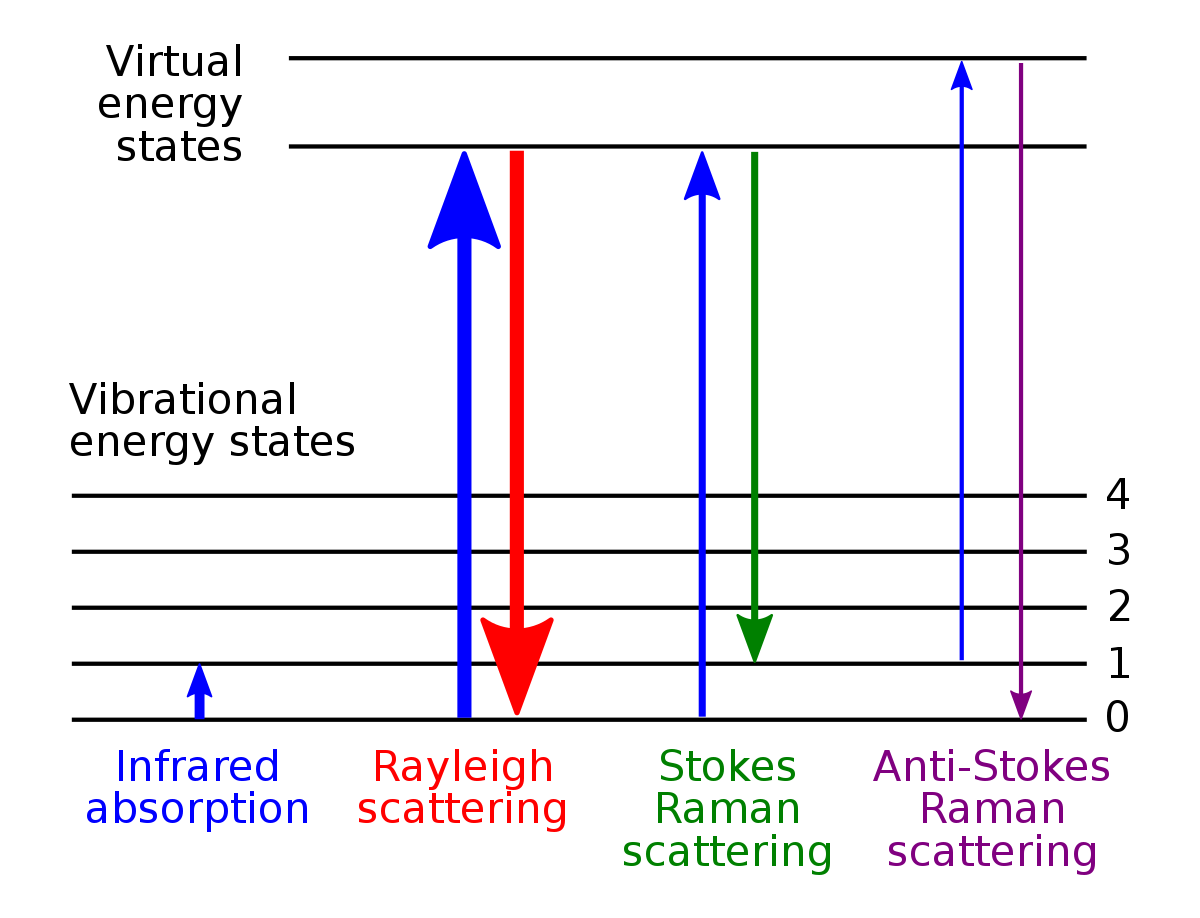
\includegraphics[width=0.4\linewidth]{Raman.png}
        \caption{Raman spectroscopic mechanics.}
        \label{fig:Raman}
    \end{figure}
    \begin{itemize}
        \item IR: Pump an electron up one vibrational mode. Sometimes multiple via overtones.
        \item Raman: Take your molecule, shoot a laser at the sample, and see what light scatters. You're least interested in \textbf{Rayleigh scattering}. What you care about is different changes (\textbf{Stokes} and \textbf{Anti-Stokes Raman scattering}). Note that the latter will be far less intense than the former due to the differences in populations between the $v=0,1$ states. We resolve vibrational energy levels by looking at differences between input and output frequency.
        \begin{itemize}
            \item Indeed, in words: Rayleigh scattering is the most intense, Stokes is ok, and Anti-Stokes is poor.
        \end{itemize}
        \item Populations are proportional to the sizes of the arrows in Figure \ref{fig:Raman}.
        \item Raman is good for materials, not for molecules.
        \begin{itemize}
            \item Great for \ce{MoS2}, but for molecules, you need huge fluxes which tend to fry your sample.
        \end{itemize}
        \item Anderson is not a huge fan of Raman spectroscopy.
        \item How Raman actually works: Your photon doesn't so much get absorbed as it scatters off of the electron cloud by coupling with the polarization wavefunction.
        \item Rayleigh is elastic; Raman is inelastic scattering.
        \item Conjugated macrocycles (e.g., heme groups) are great, but most aren't. Worth trying in the lab, but don't get your hopes up.
        \item Resonance is when you have a specific optical bond being much more intense.
    \end{itemize}
    \item To finish off our brief treatment of vibrational spectroscopy, we'll discuss isotope effects.
    \begin{itemize}
        \item Many times we want to test whether an observed vibration corresponds to specific atoms. To do this, we want to do an isotopic substitution.
        \item This can change the energy of a vibration by an amount that can be predicted by the simple harmonic oscillator approximation.
    \end{itemize}
    \item Example: Consider \ce{{}^16O2} vs. \ce{{}^18O2}.
    \begin{itemize}
        \item In Raman spectroscopy, we have $\nu_{00}=\SI{749}{\per\centi\meter}$ and $\nu_{00}=\SI{708}{\per\centi\meter}$, respectively.
        \item Recall that $\nu=k\sqrt{F/\mu}$, where
        \begin{equation*}
            \frac{1}{\mu} = \frac{1}{\ce{{}^16O}}+\frac{1}{\ce{{}^16O}}
            = \frac{\ce{{}^16O}\ce{{}^16O}}{\ce{{}^16O}+\ce{{}^16O}}
        \end{equation*}
        \item Thus,
        \begin{align*}
            \mu_{16} &= 0.125&
            \mu_{18} &= 0.111
        \end{align*}
        \item It follows that
        \begin{align*}
            \frac{\nu_{18}}{\nu_{16}} &= \frac{\sqrt{\ce{{}^18O2}}}{\sqrt{\ce{{}^16O2}}}\\
            \nu_{18} &= \frac{\sqrt{0.111}}{\sqrt{0.125}}\cdot 749\\
            \nu_{18} &\approx \SI{706}{\per\centi\meter}
        \end{align*}
        \item We'll get to practice this on the HW.
    \end{itemize}
    \item The HW will be due 1-2 weeks before the final.
    \item Further examples.
    \begin{enumerate}
        \item Test if chlorophyll photosystem II is actively producing oxygen.
        \begin{itemize}
            \item Air has regular (\ce{{}^16O2}) oxygen, so we set the photosystem up with \ce{{}^18OH2} and use IR to hopefully detect \ce{{}^18O2} being generated.
        \end{itemize}
        \item Test if a metal complex has a \ce{M#N} bond.
        \begin{itemize}
            \item Synthesize your complex with both \ce{{}^14N} and \ce{{}^15N}.
            \item Know that \ce{M#{}^14N} is approximately \SI{1000}{\per\centi\meter} and use the above to calculate that \ce{M#{}^15N} is about \SI{920}{\per\centi\meter}.
            \item Take spectra of both complexes and then subtract the two to obtain a difference spectrum. If nitrogen is being incorporated, your difference spectrum should be flat except for two peaks (one positive and one negative) at \SI{1000}{\per\centi\meter} and \SI{920}{\per\centi\meter}.
        \end{itemize}
    \end{enumerate}
    \item Last example from Anderson's written notes.
    \item \textbf{Nuclear resonance vibrational spectroscopy}: A type of vibrational spectroscopy that uses a synchrotron to induce a nuclear excitation. \emph{Also known as} \textbf{NRVS}.
    \begin{itemize}
        \item This excitation can then couple to vibrations of the excited nucleus.
        \item Particularly relevant for \ce{Fe}, the most common nucleon to study with NRVS.
        \item Related to Mossbauer spectroscopy.
    \end{itemize}
\end{itemize}




\end{document}